% vim: set tabstop=4 shiftwidth=4 expandtab :
\section{Motivation \label{sec:motivation}}

    % Representative inputs are important. Example.
    % Artificial representative input sets are hard to create
    % Representative input sets created out of real data are also hard to create
    % Just using real data online is not enough. Efficiency metrics are needed
    % We do not have a proper efficiency metric. Example.
    % The paper shows how to construct one.

    In this section we first motivate online iterative compilation by showing the deleterious effects of using non-representative input
    sets and that it is hard to create representative ones. Then we go on to examine what stops us from just using real inputs online and
    what we need to overcome the problem.

    \begin{figure}[t]
        \centering
        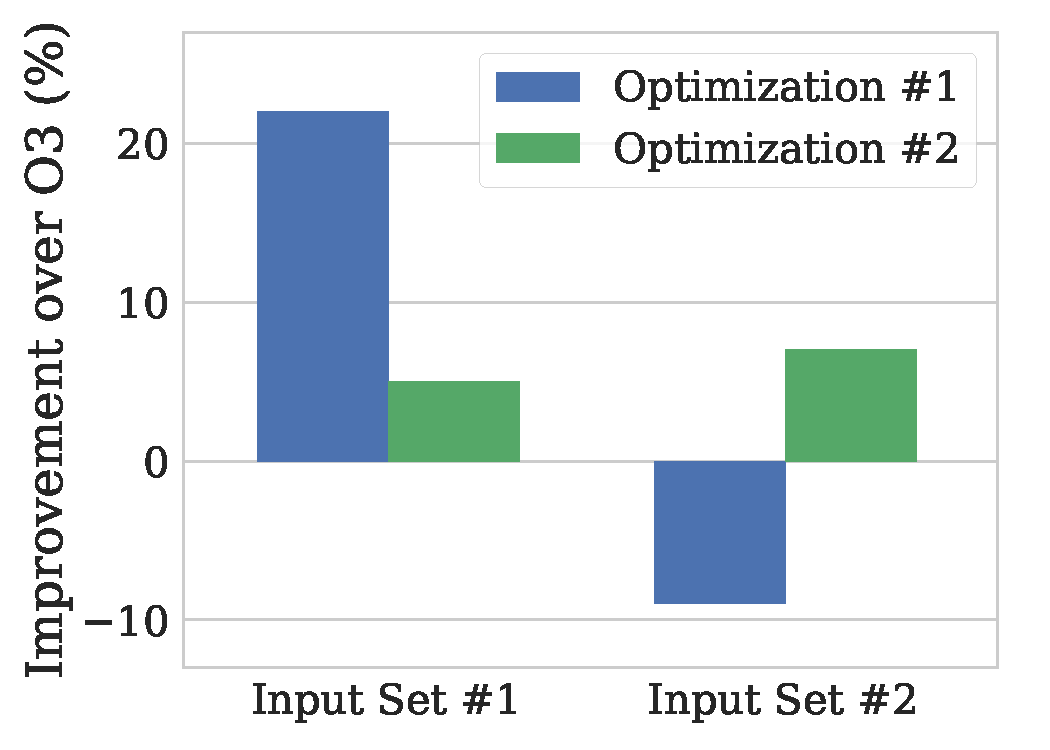
\includegraphics[width=0.7\linewidth]{figs/motivation_two_inputs.pdf}
        \caption{Average speedup over \texttt{-O3} for the \texttt{tiff2bw} benchmark when optimized with two different optimization sequences and
        evaluated on two distinct input sets. Each sequence was selected by iterative compilation on only one of the input sets. Processing
        inputs with a version optimized for a different input set produces suboptimal results, supporting that iterative compilation needs
        representative inputs.}
        \label{fig:motivation_wrong_inputs}
    \end{figure}

    \paragraph{Iterative compilation needs representative inputs.}
%%    Figure~\ref{fig:motivation_wrong_inputs} highlights what happens when we apply iterative compilation using the wrong set of inputs, we selected two distinct sets of
%%    10 out of the 1,000 inputs of the of \textit{KDataSets}~\cite{chen10,chen12a} for the \texttt{tiff2bw} benchmark.
%%    The first set represents the training set, i.e., the set of inputs that will be used for selecting the best optimization sequence by
%%    iterative compilation, and the second set is a specific set of inputs which is misrepresented by the training set, let us call it the production set.
%%    After performing iterative compilation on the training set, the selected optimization sequence has an average of 22\% improvement over -O3 for
%%    the training set itself, but it produces a slowdown of about 9\% for the production set.
%%    However, in the ideal case, if the iterative compilation was performed on the production set itself, it would be able to find an optimization sequence that
%%    results on a 7\% improvement over -O3, this is an improvement of about 17\% over
%%    the result of iterative compilation on the wrong set of inputs.

    Figure~\ref{fig:motivation_wrong_inputs} highlights what happens when we apply iterative compilation using the wrong set of inputs. We
    selected two distinct subsets of the \textit{KDataSets}~\cite{chen10,chen12a} inputs for the \texttt{tiff2bw} benchmark. Each subset
    has ten inputs. Using iterative compilation we find the best optimization sequence for each subset separately.
    Figure~\ref{fig:motivation_wrong_inputs} shows the speedup over \texttt{-O3} achieved by each sequence when using either of the two
    subsets. Optimization \#1, which was selected using input set \#1, speeds up \texttt{tiff2bw} by 22\% on average when processing set
    \#1, but hurts performance when used with set \#2. Similarly, using optimization \#2 on input set \#1 only improves performance by 5\%,
    much less than what optimization \#1 achieves. In both cases, optimizing the benchmark for the same set it will be evaluated on
    improves performance by 15\% compared to optimizing for some other set. To make iterative compilation profitable, applying it on
    inputs similar to the ones the application will be used with is absolutely necessary.


    \paragraph{Representative input sets are hard to create.} For developers to create artificial input sets, they first need to know how
    their application is actually being used. This is not always easy or even possible. Then, they need to create data that will trigger a
    similar behavior as when the application is used by users. This needs a deep knowledge of the potential user behavior and
    considerable effort. This will have to be a continuous work in progress, to handle changes in the way the application is used. In some
    areas, such as mobile computing, where developers do not traditionally optimize their applications or provide inputs for performance
    testing, depending on them to provide inputs is unrealistic.

    Collecting real input data online and processing them again offline to evaluate optimizations is not a solution either. It requires
    manual modifications to the application to save the data, more modifications to avoid side effects while reusing data, and even more
    modifications to ensure that the application does the same work every time the same data are reused, despite changes in the rest of
    the system state. \FIXME{ZW: This is a bit vague. I think we need an example to illustrate why the application may not perform the same
    work if the same input is used.}
    This is significant engineering work. Even if this was not the case, many applications are just not able to save
    data for privacy or storage overhead reasons. \FIXME{Refs?}

    \paragraph{Using live inputs online is not enough.} We could overcome the problem of representative inputs by just evaluating
    optimization sequences online while the application is being used. This gives us live data but creates a bigger problem, that we cannot
    compare different optimizations just by runtime anymore. When optimizations are tested against the same inputs, determining their
    relative efficiency is just a matter of comparing runtimes. A shorter runtime for the same work means a more efficient binary.
    With live data, we cannot do this, the binary processes whatever the input happens to be. Larger inputs require more work and will
    likely lead to longer execution times, regardless of optimizations.

    As an example, consider a sorting algorithm. To measure the efficiency of an optimization for the algorithm, we need to look at not just
    how long the algorithm runs but also how many items it processes per run. Just comparing the runtimes of two invocations does not
    provide any information about efficiency, as the two invocations may not process the same number of items. We need another efficiency metric
    that only requires a single execution of an optimized binary with a single input.

    \paragraph{Existing efficiency metrics are not up to the task.} Application-specific efficiency metrics~\cite{alameldeen06,coppa14} may
    work well, but the developer has to choose the appropriate metric and then manually modify the application to calculate it. Speedup
    over a common baseline binary is an adequate application-agnostic metric but it cannot be used online. It requires measuring runtime
    for each input twice, one with the baseline and one with the optimized binary.

    Typical single-run performance metrics, like runtime or Instructions Per Cycle~(IPC), are not fit for purpose. To show this, we
    performed iterative compilation on \texttt{tiff2bw}, evaluating each optimization sequence on a different input and using either
    runtime or IPC as our efficiency metric. We selected a set of ten inputs from the KDataSets. When
    iterative compilation is driven by runtime, the selected optimization slows down the benchmark by 3\% compared to \texttt{-O3}. When
    driven by IPC, it is even worse with an average slowdown of 49\%. Its very high IPC of 3.25 does not indicate high performance. The
    actual best optimization over the whole input set improves performance by 7\% while only having an average IPC of 2.31.
    When the binary changes, higher IPC does not necessarily mean better performance, different optimizations affect IPC in different ways.
    Similarly, when the input changes, shorter runtimes do not mean faster execution, it may just be that processing the input requires less work. 

\begin{table}[t]
\centering
\label{tab:motivation_metrics}
\begin{tabular}{|l|l|l|}
\hline
\textbf{Metric} & \textbf{Speedup/Slowdown} & \textbf{IPC} \\ \hline
\rowcolor{Gray} Oracle (Speedup)             & 7\% speedup                                 & 2.31                      \\ \hline
IPC                          & 49\% slowdown                                & 3.25                      \\ \hline
\rowcolor{Gray}1/Runtime                    & 3\% slowdown                                  & {-}   \\ \hline
\end{tabular}
\caption{Comparison of iterative compilation guided by different metrics.
The oracle is guided by the average speedup over \texttt{-O3} on all inputs.
For IPC and runtime, each optimization was evaluated on a different input.
}
\end{table}

%    \begin{figure}[t]
%        \centering
%        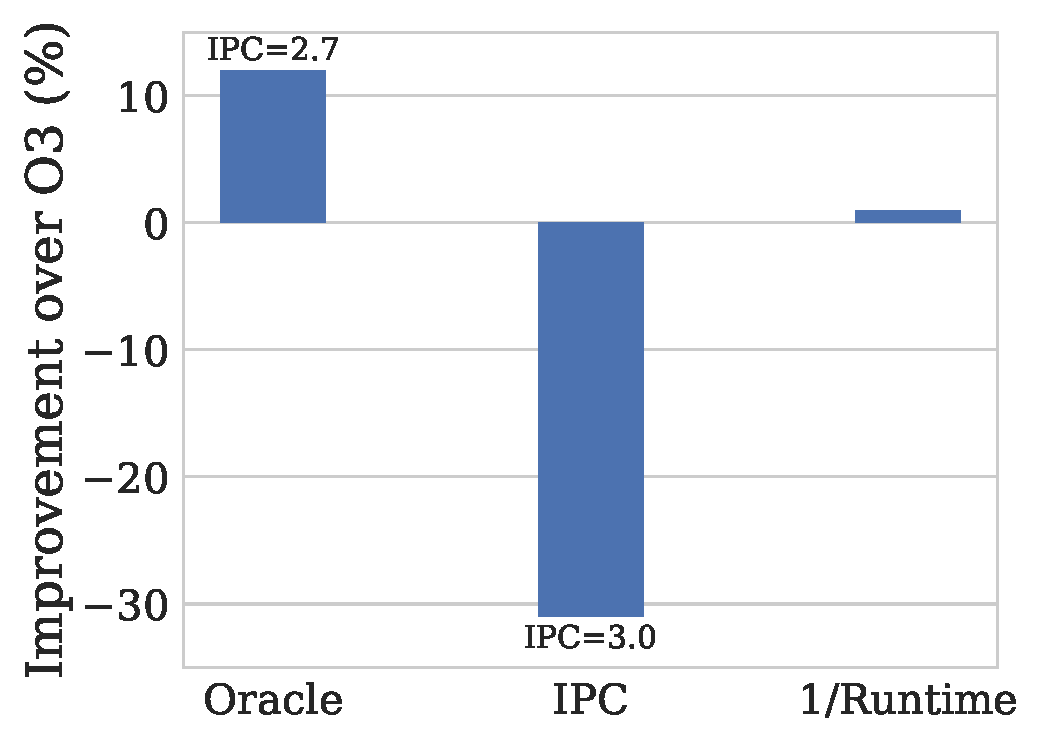
\includegraphics[width=0.7\linewidth]{figs/motivation_metrics.pdf}
%        \caption{Average speedup over \texttt{-O3} for the \texttt{tiff2bw} benchmark when optimized with two different optimization sequences and
%        evaluated on two distinct input sets. Each sequence was selected by iterative compilation on only one of the input sets. Processing
%        inputs with a version optimized for a different input set produces suboptimal results, supporting that iterative compilation needs
%        representative inputs.}
%        \label{fig:motivation_metrics}
%    \end{figure}




%     \FIXME{Evidence2:}
%    To show this, we ran
%    each of the \FIXME{32} \textit{KDataSets} benchmarks 1,000 times, each time with a different input \textit{and} a different optimized
%    binary, and we measured three metrics: runtime, inverse runtime, and IPC. \FIXME{Fig.XXX} shows the correlation coefficient between
%    them and a reasonable efficiency metric, speedup over \texttt{-O0}. For all benchmarks, the correlation coefficient is below
%    \FIXME{0.20} for runtime and below \FIXME{0.35} for inverse runtime. Both have obvious reasons for being inappropriate efficiency
%    metrics. Doubling the amount of data to be processed will cause the runtime to rise and the inverse runtime to fall, even if we use the same binary.
%    Efficiency has nothing to do with it. IPC also correlates poorly with efficiency, the correlation coefficient being just \FIXME{0.15}.
%    While it is used often in computer architecture, it works there because it is used with invariant binaries. In contrast, any compiler
%    optimization that trades high latency instructions for multiple low latency instructions can reduce IPC while improving efficiency.
    No existing metric can give us an application-agnostic measure of efficiency with a single execution. Without one, online iterative
    compilation is impossible. Without doing it online, iterative compilation will always be limited by the quality of the input set.
    The rest of the paper will show how to create an appropriate efficiency metric and how to use it for true online iterative
    compilation.

%\begin{figure*}[t]
%    \centering
%    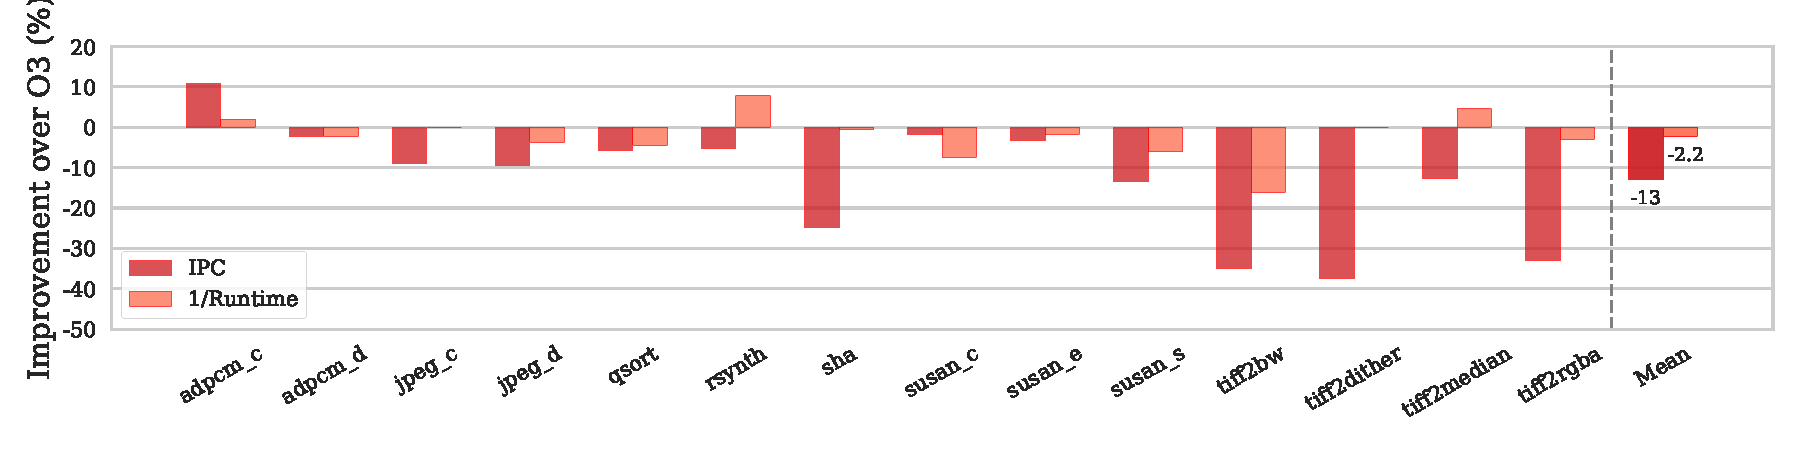
\includegraphics[width=\textwidth]{figs/motivation-speedups.pdf}
%    \caption{\FIXME{[Fall-back Result]} Performance improvement of iterative compilation guided by IPC and runtime.}
%    \label{fig:motivation-speedups}
%\end{figure*}
